% (c) 2026 Stephanie Märklin, OST Ostschweizer Fachhochschule
%
% !TEX root = ../../buch.tex
% !TEX encoding = UTF-8
%
% Rolle im Paper: Das Ergebnis der Rechnung formulieren und mathematisch deuten
%
% Stichworte:
% 17.5 Interpretation der Eigenwerte (Vorspann)
% - Andocken: die Rechnung liefert vier Zahlen -- jetzt ihre Deutung
% - Fahrplan: Real- und Imaginärteil, dann das komplexe Paar der
%   Dutch Roll
%
% 17.5.1 Realteil und Imaginärteil
% - Eigenwert zerlegen: lambda = sigma + i omega
% - e^{lambda t} in zwei Faktoren; Euler zitieren (Buchteil, DGL)
% - benennen: e^{sigma t} = Dämpfung (Vorzeichen offen),
%   Klammer = Schwingung mit Frequenz omega
% - Abbildung: drei Fälle sigma < 0, = 0, > 0 (TikZ aus Folien)
% - allgemeine Lösung als Linearkombination der vier Basislösungen;
%   Störung legt Anteile fest
% - keine Bewertung, kein Kriterium als Formel (Mechanik + Resultat)
%
% 17.5.2 Das komplexe Eigenwertpaar der Dutch Roll
% - reelle Matrix -> konjugierte Paare
% - Paar setzt sich zur reellen Schwingung zusammen (Buchteil)
% - reeller Eigenwert vs. komplexes Paar
% - Dutch Roll = komplexes Paar; klingt genau dann ab, wenn sigma < 0

\section{Interpretation der Eigenwerte
\label{aircraft:section:5-interpretation}}
\kopfrechts{Interpretation}
Die Rechnung des letzten Abschnitts liefert vier Zahlen.
In diesem Abschnitt deuten wir sie.
Wir betrachten zuerst Real- und Imaginärteil eines einzelnen
Eigenwerts, danach das komplexe Eigenwertpaar der Dutch Roll.

\subsection{Realteil und Imaginärteil
\label{aircraft:subsection:realteil-imaginaerteil}}
Wir schreiben einen Eigenwert als
\begin{equation}
    \lambda
    =
    \sigma + i\omega
    \label{aircraft:eqn:zerlegung}
\end{equation}
mit dem Realteil $\sigma$ und dem Imaginärteil $\omega$.
Die zugehörige Lösung zerfällt in zwei Faktoren,
\begin{equation}
    e^{\lambda t}
    =
    e^{\sigma t} \cdot e^{i\omega t}.
    \label{aircraft:eqn:faktoren}
\end{equation}
Wir setzen $\omega t$ in die eulersche Formel aus
Satz~\ref{buch:holomorph:holomorph:satz:eulerformel} ein und erhalten
\begin{equation}
    e^{\lambda t}
    =
    e^{\sigma t} (\cos\omega t + i\sin\omega t).
    \label{aircraft:eqn:euler}
\end{equation}
Der Realteil $\sigma$ heisst \emph{Dämpfung} (damping),
der Imaginärteil $\omega$ \emph{Frequenz} (frequency).
Die Abbildung~\ref{aircraft:fig:eigenwerte} zeigt den Verlauf der Lösung für
die drei Fälle $\sigma < 0$, $\sigma = 0$ und $\sigma > 0$.
Die gestrichelte Kurve ist die \emph{Hüllkurve} (envelope) $e^{\sigma t}$,
welche die Schwingung von oben einschliesst.
Für $\sigma < 0$ fällt die Hüllkurve gegen null.
Die Schwingung klingt ab, und das Flugzeug kehrt in die Ruhelage zurück.
Dieser Fall heisst stabil.
Für $\sigma = 0$ ist die Hüllkurve konstant.
Die Schwingung klingt weder ab noch schaukelt sie sich auf, und das Flugzeug
bleibt in der Nähe der Ruhelage.
Dieser Fall heisst \emph{indifferent}.
Für $\sigma > 0$ wächst die Hüllkurve.
Die Schwingung schaukelt sich auf, und das Flugzeug entfernt sich
von der Ruhelage.
Dieser Fall heisst instabil.
Der Name Dämpfung gilt also mit Vorzeichen.
Im instabilen Fall spricht man von negativer Dämpfung.
Die Stabilität nach Abschnitt~\ref{aircraft:section:3-mathematische-stabilitaet}
verlangt,
dass die Lösung gegen $\vec 0$ geht.
Das ist genau dann der Fall, wenn $\sigma < 0$ ist.
Das Vorzeichen des Realteils entscheidet also über die Stabilität.

\begin{figure}
    \centering
    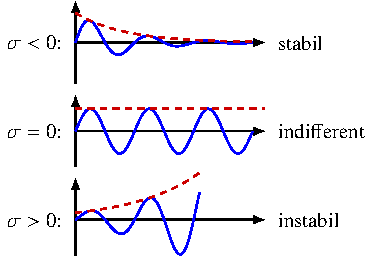
\includegraphics{papers/aircraft/images/eigenwerte.pdf}
    \caption{Verlauf der Lösung $e^{\lambda t}$ in den drei Fällen
    stabil ($\sigma < 0$), indifferent ($\sigma = 0$) und instabil ($\sigma > 0$).
    Die gestrichelte Kurve ist die Hüllkurve $e^{\sigma t}$.
    \label{aircraft:fig:eigenwerte}}
\end{figure}

Zwei Zeiten charakterisieren die Schwingung, die Periode $T$ und die
Halbwertszeit $t_{1/2}$.
Die \emph{Periode} (period) ist die Dauer einer vollen Schwingung.
Aus $\omega T = 2\pi$ folgt $T = 2\pi/\omega$.
Die \emph{Halbwertszeit} (time to half amplitude) ist die Zeit, nach der die
Hüllkurve $e^{\sigma t}$ auf die Hälfte gefallen ist.
Aus $e^{\sigma t_{1/2}} = \frac{1}{2}$ folgt
\begin{equation}
    t_{1/2}
    =
    -\frac{\ln 2}{\sigma}.
    \label{aircraft:eqn:halbwertszeit}
\end{equation}
Für $\sigma < 0$ ist die Halbwertszeit positiv und gibt an, wie rasch eine
Störung abklingt.
Für $\sigma > 0$ ist die Halbwertszeit negativ, denn die Hüllkurve fällt nie auf
die Hälfte, sondern wächst.
Der Betrag $|t_{1/2}| = \ln 2/\sigma$ ist dann die Zeit, in der die Hüllkurve
auf das Doppelte anwächst.
Diese Zeit heisst \emph{Verdoppelungszeit} (time to double amplitude).
Je grösser die Verdoppelungszeit ist, desto schwächer ist die Instabilität.
Entsprechend ist die Stabilität umso schwächer, je grösser die Halbwertszeit
ist.
Eine grosse Verdoppelungszeit lässt dem Piloten viel Zeit, eine Störung von
Hand zu korrigieren.

Die allgemeine Lösung der Bewegungsgleichung ist eine
Linearkombination der vier Lösungen $\vec{x}_0^{(k)} e^{\lambda_k t}$,
und die Störung legt die Anteile fest.

\subsection{Das komplexe Eigenwertpaar der Dutch Roll
\label{aircraft:subsection:eigenwertpaar}}
Die Systemmatrix ist reell, also treten komplexe Eigenwerte als
konjugierte Paare $\sigma \pm i\omega$ auf.
Die beiden Lösungen eines Paars setzen sich nach
Kapitel~\ref{chapter:differentialgleichungen} zur reellen Schwingung
$e^{\sigma t}\cos\omega t$ zusammen.
Ein reeller Eigenwert beschreibt eine Bewegung ohne Schwingung, ein
komplexes Paar eine Schwingung mit der Dämpfung $\sigma$ und der
Frequenz $\omega$.
Die Dutch Roll ist ein komplexes Eigenwertpaar.
Sie klingt genau dann ab, wenn $\sigma < 0$ ist.

\subsection{Die Eigenvektoren
\label{aircraft:section:5-eigenvektoren}}
Bisher haben wir nur die Eigenwerte gedeutet.
Die Lösung \eqref{aircraft:eqn:exponentialansatz} enthält aber auch den
Eigenvektor $\vec x_0$.
Der Eigenvektor ist ein Zustand, der sich unter dem Bewegungsgesetz nur um
den Faktor $e^{\lambda t}$ verändert.
Die Verhältnisse seiner vier Komponenten bleiben also erhalten.
Die Komponenten geben deshalb an, mit welcher Amplitude der Schiebewinkel, die
Rollrate, die Gierrate und der Rollwinkel an der Lösung beteiligt sind.
Eine Lösung $\vec x_0 e^{\lambda t}$ heisst \emph{Eigenbewegung} (mode).
Bei einem komplexen Eigenwert $\lambda$ hat die Gleichung
\eqref{aircraft:eqn:eigenwertgleichung-homogen} komplexe Koeffizienten, und der
Eigenvektor ist deshalb ebenfalls komplex.
Für den Vergleich der Komponenten verwenden wir dann ihre Beträge.

Am Eigenvektor lässt sich ablesen, welche Zustandsgrössen eine Eigenbewegung
betrifft.
Ist eine Komponente von $\vec x_0$ gross und sind die übrigen klein, so
betrifft die Eigenbewegung fast nur eine Zustandsgrösse.
Sind alle Komponenten von vergleichbarer Grösse, so sind alle Zustandsgrössen
beteiligt, und die Eigenbewegung ist gekoppelt im Sinne von
Abschnitt~\ref{aircraft:section:2-dynamisches-system}.
Wäre die Systemmatrix $A$ eine Diagonalmatrix, so wären die Eigenvektoren die
Einheitsvektoren, und keine Eigenbewegung wäre gekoppelt.